\subsection{Extreme-gate-length output characteristics and potential maps}
\label{sec:part2_remaining}
To complete the Chapter 4 Part 2 comparisons, the original SProcess geometries
were reused in a separate project copy, with $L_G=52$ or $1002$ nm and
$T_{\mathrm{SI}}=10$ or $30$ nm. Four SDevice runs generated 28 successful
$I_D$--$V_D$ curves: seven $V_{GS}$ biases ($0,0.2,\ldots,1.2$ V)
for each of the four devices, over $V_{DS}=0$ to $1.2$ V in
$0.04$ V steps. The original data comprise 31 points per curve,
and the display CSVs retain 11 exact points per curve without fitting.
A solid line denotes $L_G=52$ nm and a dashed line $L_G=1002$ nm;
matching colors denote equal $V_{GS}$ biases.
For legibility these output-current ordinates are multiplied by
$10^3$ relative to the simulator-exported current magnitudes;
the conversion is an explicit display scaling \emph{only},
not an assumption that the native 2D current is in amperes.

\begin{figure}[H]\centering
\begin{tikzpicture}
\begin{axis}[width=.95\linewidth,height=7.1cm,
xlabel={$V_{DS}$ (V)},ylabel={$10^3 I_D$ (scaled exported units)},
xmin=0,xmax=1.2,ymin=0,
grid=both,
legend style={font=\scriptsize,at={(0.02,0.98)},anchor=north west,fill opacity=.9,text opacity=1},
legend cell align=left]
\addplot+[no marks,thick,forget plot,solid,color=black] table[col sep=comma,x=VDS_V,y=LG52_VGS00_mA_assuming_A] {data/part2_idvd_tsi30_sampled.csv};
\addplot+[no marks,thick,forget plot,solid,color=red!85!black] table[col sep=comma,x=VDS_V,y=LG52_VGS02_mA_assuming_A] {data/part2_idvd_tsi30_sampled.csv};
\addplot+[no marks,thick,forget plot,solid,color=orange!90!black] table[col sep=comma,x=VDS_V,y=LG52_VGS04_mA_assuming_A] {data/part2_idvd_tsi30_sampled.csv};
\addplot+[no marks,thick,forget plot,solid,color=green!60!black] table[col sep=comma,x=VDS_V,y=LG52_VGS06_mA_assuming_A] {data/part2_idvd_tsi30_sampled.csv};
\addplot+[no marks,thick,forget plot,solid,color=cyan!70!black] table[col sep=comma,x=VDS_V,y=LG52_VGS08_mA_assuming_A] {data/part2_idvd_tsi30_sampled.csv};
\addplot+[no marks,thick,forget plot,solid,color=blue] table[col sep=comma,x=VDS_V,y=LG52_VGS10_mA_assuming_A] {data/part2_idvd_tsi30_sampled.csv};
\addplot+[no marks,thick,forget plot,solid,color=magenta!85!black] table[col sep=comma,x=VDS_V,y=LG52_VGS12_mA_assuming_A] {data/part2_idvd_tsi30_sampled.csv};
\addplot+[no marks,thick,forget plot,dashed,color=black] table[col sep=comma,x=VDS_V,y=LG1002_VGS00_mA_assuming_A] {data/part2_idvd_tsi30_sampled.csv};
\addplot+[no marks,thick,forget plot,dashed,color=red!85!black] table[col sep=comma,x=VDS_V,y=LG1002_VGS02_mA_assuming_A] {data/part2_idvd_tsi30_sampled.csv};
\addplot+[no marks,thick,forget plot,dashed,color=orange!90!black] table[col sep=comma,x=VDS_V,y=LG1002_VGS04_mA_assuming_A] {data/part2_idvd_tsi30_sampled.csv};
\addplot+[no marks,thick,forget plot,dashed,color=green!60!black] table[col sep=comma,x=VDS_V,y=LG1002_VGS06_mA_assuming_A] {data/part2_idvd_tsi30_sampled.csv};
\addplot+[no marks,thick,forget plot,dashed,color=cyan!70!black] table[col sep=comma,x=VDS_V,y=LG1002_VGS08_mA_assuming_A] {data/part2_idvd_tsi30_sampled.csv};
\addplot+[no marks,thick,forget plot,dashed,color=blue] table[col sep=comma,x=VDS_V,y=LG1002_VGS10_mA_assuming_A] {data/part2_idvd_tsi30_sampled.csv};
\addplot+[no marks,thick,forget plot,dashed,color=magenta!85!black] table[col sep=comma,x=VDS_V,y=LG1002_VGS12_mA_assuming_A] {data/part2_idvd_tsi30_sampled.csv};
\addlegendimage{thick,solid,color=black}\addlegendentry{$V_{GS}=0.0$ V}
\addlegendimage{thick,solid,color=red!85!black}\addlegendentry{$V_{GS}=0.2$ V}
\addlegendimage{thick,solid,color=orange!90!black}\addlegendentry{$V_{GS}=0.4$ V}
\addlegendimage{thick,solid,color=green!60!black}\addlegendentry{$V_{GS}=0.6$ V}
\addlegendimage{thick,solid,color=cyan!70!black}\addlegendentry{$V_{GS}=0.8$ V}
\addlegendimage{thick,solid,color=blue}\addlegendentry{$V_{GS}=1.0$ V}
\addlegendimage{thick,solid,color=magenta!85!black}\addlegendentry{$V_{GS}=1.2$ V}
\end{axis}
\end{tikzpicture}
\caption{Sentaurus SOI output curves at $T_{\mathrm{SI}}=30$ nm.
$L_G=52$ nm (solid) and $L_G=1002$ nm (dashed);
each color is a gate bias from 0 to 1.2 V.
Eleven unmodified samples per curve from the original 31 are plotted.}
\label{fig:part2_idvd_tsi30}
\end{figure}

\begin{figure}[H]\centering
\begin{tikzpicture}
\begin{axis}[width=.95\linewidth,height=7.1cm,
xlabel={$V_{DS}$ (V)},ylabel={$10^3 I_D$ (scaled exported units)},
xmin=0,xmax=1.2,ymin=0,
grid=both,
legend style={font=\scriptsize,at={(0.02,0.98)},anchor=north west,fill opacity=.9,text opacity=1},
legend cell align=left]
\addplot+[no marks,thick,forget plot,solid,color=black] table[col sep=comma,x=VDS_V,y=LG52_VGS00_mA_assuming_A] {data/part2_idvd_tsi10_sampled.csv};
\addplot+[no marks,thick,forget plot,solid,color=red!85!black] table[col sep=comma,x=VDS_V,y=LG52_VGS02_mA_assuming_A] {data/part2_idvd_tsi10_sampled.csv};
\addplot+[no marks,thick,forget plot,solid,color=orange!90!black] table[col sep=comma,x=VDS_V,y=LG52_VGS04_mA_assuming_A] {data/part2_idvd_tsi10_sampled.csv};
\addplot+[no marks,thick,forget plot,solid,color=green!60!black] table[col sep=comma,x=VDS_V,y=LG52_VGS06_mA_assuming_A] {data/part2_idvd_tsi10_sampled.csv};
\addplot+[no marks,thick,forget plot,solid,color=cyan!70!black] table[col sep=comma,x=VDS_V,y=LG52_VGS08_mA_assuming_A] {data/part2_idvd_tsi10_sampled.csv};
\addplot+[no marks,thick,forget plot,solid,color=blue] table[col sep=comma,x=VDS_V,y=LG52_VGS10_mA_assuming_A] {data/part2_idvd_tsi10_sampled.csv};
\addplot+[no marks,thick,forget plot,solid,color=magenta!85!black] table[col sep=comma,x=VDS_V,y=LG52_VGS12_mA_assuming_A] {data/part2_idvd_tsi10_sampled.csv};
\addplot+[no marks,thick,forget plot,dashed,color=black] table[col sep=comma,x=VDS_V,y=LG1002_VGS00_mA_assuming_A] {data/part2_idvd_tsi10_sampled.csv};
\addplot+[no marks,thick,forget plot,dashed,color=red!85!black] table[col sep=comma,x=VDS_V,y=LG1002_VGS02_mA_assuming_A] {data/part2_idvd_tsi10_sampled.csv};
\addplot+[no marks,thick,forget plot,dashed,color=orange!90!black] table[col sep=comma,x=VDS_V,y=LG1002_VGS04_mA_assuming_A] {data/part2_idvd_tsi10_sampled.csv};
\addplot+[no marks,thick,forget plot,dashed,color=green!60!black] table[col sep=comma,x=VDS_V,y=LG1002_VGS06_mA_assuming_A] {data/part2_idvd_tsi10_sampled.csv};
\addplot+[no marks,thick,forget plot,dashed,color=cyan!70!black] table[col sep=comma,x=VDS_V,y=LG1002_VGS08_mA_assuming_A] {data/part2_idvd_tsi10_sampled.csv};
\addplot+[no marks,thick,forget plot,dashed,color=blue] table[col sep=comma,x=VDS_V,y=LG1002_VGS10_mA_assuming_A] {data/part2_idvd_tsi10_sampled.csv};
\addplot+[no marks,thick,forget plot,dashed,color=magenta!85!black] table[col sep=comma,x=VDS_V,y=LG1002_VGS12_mA_assuming_A] {data/part2_idvd_tsi10_sampled.csv};
\addlegendimage{thick,solid,color=black}\addlegendentry{$V_{GS}=0.0$ V}
\addlegendimage{thick,solid,color=red!85!black}\addlegendentry{$V_{GS}=0.2$ V}
\addlegendimage{thick,solid,color=orange!90!black}\addlegendentry{$V_{GS}=0.4$ V}
\addlegendimage{thick,solid,color=green!60!black}\addlegendentry{$V_{GS}=0.6$ V}
\addlegendimage{thick,solid,color=cyan!70!black}\addlegendentry{$V_{GS}=0.8$ V}
\addlegendimage{thick,solid,color=blue}\addlegendentry{$V_{GS}=1.0$ V}
\addlegendimage{thick,solid,color=magenta!85!black}\addlegendentry{$V_{GS}=1.2$ V}
\end{axis}
\end{tikzpicture}
\caption{Sentaurus SOI output curves at $T_{\mathrm{SI}}=10$ nm.
$L_G=52$ nm (solid) and $L_G=1002$ nm (dashed);
each color is a gate bias from 0 to 1.2 V.
Eleven unmodified samples per curve from the original 31 are plotted.}
\label{fig:part2_idvd_tsi10}
\end{figure}

\paragraph{Quantitative comparison.}
At $V_{GS}=V_{DS}=1.2$ V, the drain current in the 30-nm film is
$1.35421\times10^{-3}$ for $L_G=52$ nm versus
$2.25493\times10^{-4}$ for $L_G=1002$ nm, in the
raw exported current units. The corresponding values in the
10-nm film are $1.21289\times10^{-3}$ and
$2.32708\times10^{-4}$. At $V_{GS}=0$, $V_{DS}=1.2$ V,
the 52-nm device OFF currents are $1.08052\times10^{-4}$
(30-nm film) and $3.60182\times10^{-6}$ (10-nm film):
reducing $T_{\mathrm{SI}}$ lowers this current by about $30.0$ times,
with a $10.4\%$ reduction in the corresponding ON current.
These results support improved electrostatic control in the thinner film
but reveal an ON-current trade-off. Current-width normalization is not independently established;
therefore the figure and comparisons do not claim absolute mA units.

\paragraph{2D electrostatic potential at $V_{GS}=0$, $V_{DS}=1.2$ V.}
The 52-nm devices also produced the saved SDevice snapshots
\texttt{part2\_potential\_vg00\_vd12\_n3\_des.tdr}
($T_{\mathrm{SI}}=30$ nm) and
\texttt{part2\_potential\_vg00\_vd12\_n17\_des.tdr}
($T_{\mathrm{SI}}=10$ nm).
The original Sentaurus Visual contour field is
\texttt{ElectrostaticPotential}, with the same
linear color range $[-0.287537,1.79331]$ V for both images and
identical display limits $X=[-0.18,0.18]$ $\mu$m,
$Y=[-0.40,0.08]$ $\mu$m.

\begin{figure}[H]\centering
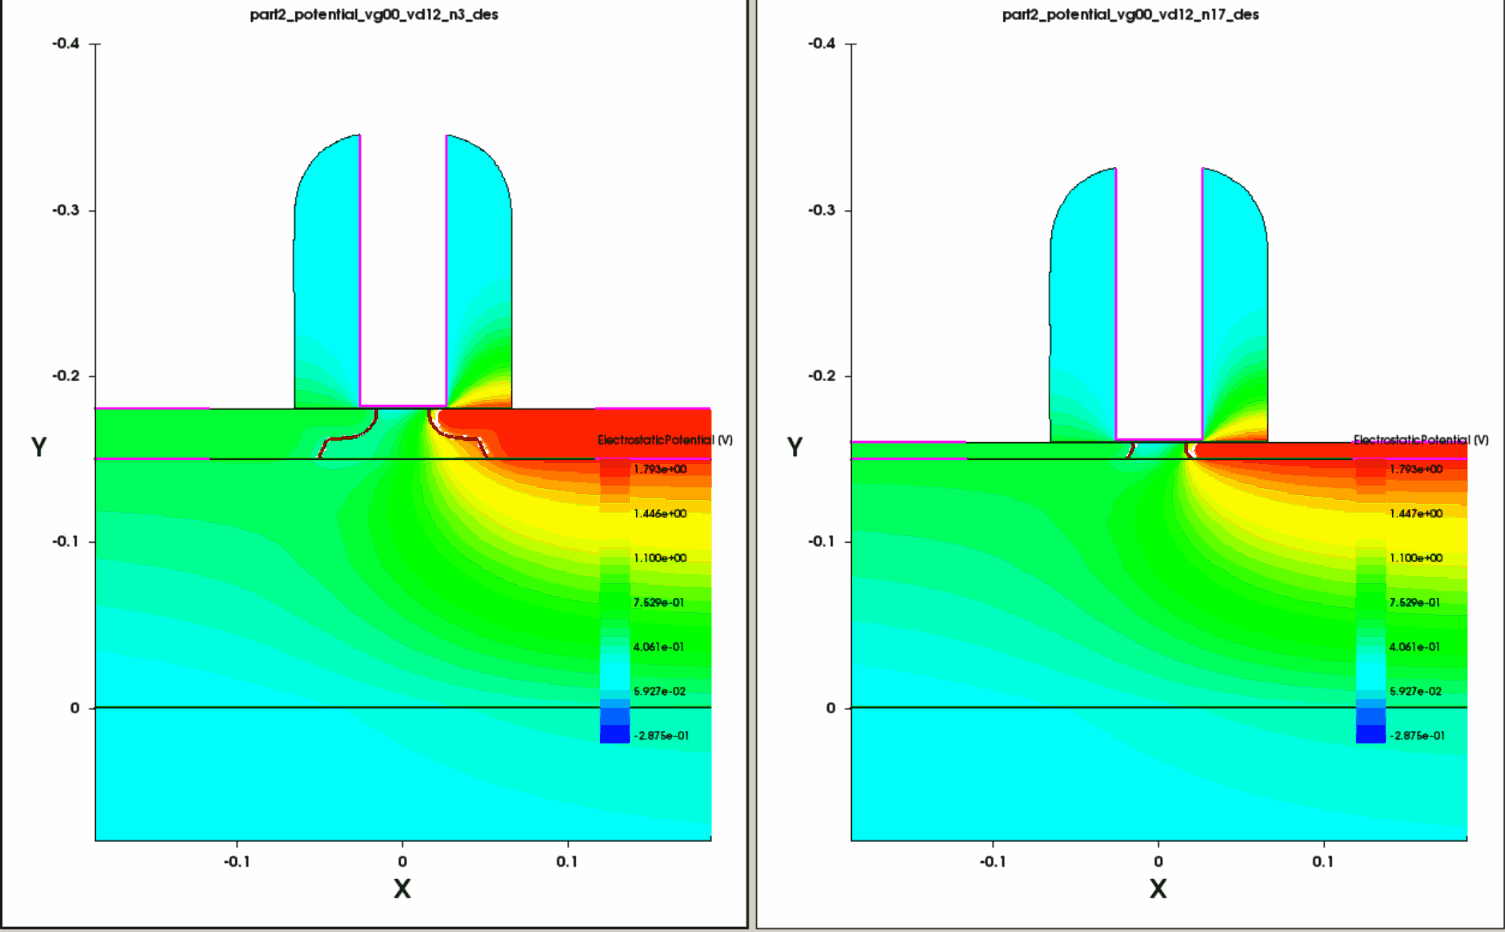
\includegraphics[width=.98\linewidth]{figures/part2_potential_comparison.png}
\caption{2D electrostatic potential at $L_G=52$ nm,
$V_{GS}=0$ V, $V_{DS}=1.2$ V. Left: $T_{\mathrm{SI}}=30$ nm;
right: $T_{\mathrm{SI}}=10$ nm. Both panels use the same
voltage scale and X/Y viewing window.}
\label{fig:part2_electrostatic_comparison}
\end{figure}

The drain-side potential extends toward the channel in both structures,
but the difference between the maps is consistent with the thinner
film's lower OFF current and DIBL from the electrical extractions.
A potential contour map alone does not establish fully depleted
operation: assessing vertical charge and energy-band distributions
provides stronger evidence (Part 5).
